\documentclass{article}

\usepackage[italian]{babel}     %testi autogenerati italiano
\usepackage{minted}             %per codice vhdl bello
\usepackage{tikz}               %per disegno fsm
\usetikzlibrary{automata, positioning, arrows}
\usepackage{circuitikz}         %per disegno componente
\usepackage{graphicx}           %per importare immagini
\usepackage{geometry}           %per gestire margini e spostamenti
\geometry {
    top=20mm,
    bmargin=20mm,
}
\usepackage{array}              %per colonne di width fissata
\usepackage{subcaption}         %tabelle divise
\usepackage{hyperref}           %links
\hypersetup{
    colorlinks=true,
    linkcolor=black,
    urlcolor=blue
}
%\usepackage[bottom]{footmisc}   %footnotes fissate a piè pagina
\usepackage{booktabs}           %per tabitem in tabular
\newcommand{\tabitem}{~~\llap{\textbullet}~~}
\renewcommand*{\thefootnote}{[\arabic{footnote}]}

\begin{document}

\setlength\parindent{0pt} %noindent automatico
\setlength\parskip{1em}

\begin{titlepage}
    \centering
    \hrule

    \vspace{0,5cm}
    {
        \normalsize Politecnico di Milano\\
        Dipartimento di Elettronica, Informazione e Bioingegneria
    }

    \vspace{5cm}
    {\Huge \textbf{Progetto di Reti Logiche\\
            2021/22}\\}

    \vspace{0,5cm}
    \large {Prof. Palermo Gianluca}

    \vspace{5cm}
    {
        \large
        \begin{tabular}{c c}
            Dario Simoni \\
            (Codice Persona: 10697990, Matricola: 932957) \\
        \end{tabular}

    }

    \vspace{6.5cm}


    \hrule

\end{titlepage}

\pagebreak

\tableofcontents

\pagebreak

\section{Requisiti di progetto} %1
\subsection{Descrizione del problema} %1.1
Si vuole realizzare un modulo HW (descritto in VHDL) che si interfacci con una memoria e che
ricevendo in ingresso un flusso continuo X da 1 bit restituisca un nuovo flusso continuo Y da 1 bit.
\par
Il flusso continuo X è generato da una seguenza continua di parole serializzate in base alla specifica, mentre il flusso continuo Y restituisce il doppio dei bit rispetto al flusso X.
\vspace{0,2cm} %un po' di spazio

\subsection{Interfaccia del componente} %1.2
Il componente da descrivere deve avere la seguente interfaccia

\begin{minted}{vhdl}
    entity project_reti_logiche is
	  port (
	    i_clk     : in  std_logic;
	    i_rst     : in  std_logic; 
	    i_start   : in  std_logic; 
	    i_data    : in  std_logic_vector (7 downto 0);
	    o_address : out std_logic_vector (15 downto 0);
    	o_done    : out std_logic; 
    	o_en      : out std_logic;
	    o_we      : out std_logic;
	    o_data    : out std_logic_vector (7 downto 0) 
	  );
    end project_reti_logiche;
\end{minted}
\vspace{0,2cm} %un po' di spazio

In particolare:
\begin{itemize}
    \item   il nome del modulo deve essere project\_reti\_logiche;
    \item   \texttt{i\_clk} è il segnale di CLOCK in ingresso generato dal TestBench;
    \item   \texttt{i\_rst} è il segnale di RESET che inizializza la macchina pronta per ricevere il primo segnale di START;
    \item   \texttt{i\_start} è il segnale di START generato dal Test Bench;
    \item   \texttt{i\_data} è il segnale (vettore) che arriva dalla memoria in seguito a una richiesta di lettura;
    \item   \texttt{o\_address} è il segnale (vettore) di uscita che manda l’indirizzo alla memoria;
    \item   \texttt{o\_done} è il segnale di uscita che comunica la fine dell’elaborazione e il dato di uscita scritto in memoria;
    \item   \texttt{o\_en} è il segnale di ENABLE da mandare alla memoria per poter comunicare (sia in lettura che in scrittura);
    \item   \texttt{o\_we} è il segnale di WRITE ENABLE da mandare alla memoria (\texttt{=1}) per poter scriverci. Per leggere da memoria esso deve essere \texttt{0};
    \item   \texttt{o\_data} è il segnale (vettore) di uscita dal componente verso la memoria.
\end{itemize}

\pagebreak

\vspace{0,2cm}

\subsection{Descrizione della memoria e dell'interazione con il componente} %1.3
Il modulo riceve in ingresso una sequenza continua di W parole, ognuna di 8 bit, e
restituisce in uscita una sequenza continua di Z parole, ognuna da 8 bit. Ognuna delle
parole di ingresso viene serializzata; in questo modo viene generato un flusso continuo U da
1 bit. Su questo flusso viene applicato il codice convoluzionale ½ (ogni bit viene codificato
con 2 bit); questa operazione genera in uscita un
flusso continuo Y. Il flusso Y è ottenuto come concatenamento alternato dei due bit di uscita.
Utilizzando la notazione riportata in figura, il bit uk genera i bit p1k e p2k che sono poi
concatenati per generare un flusso continuo yk (flusso da 1 bit). La sequenza d’uscita Z è la
parallelizzazione, su 8 bit, del flusso continuo yk
\vspace{0,3cm}

\begin{center}
    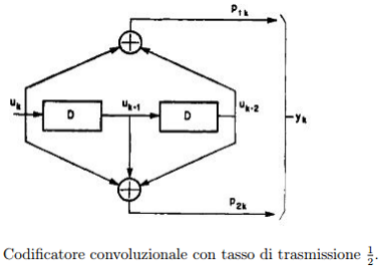
\includegraphics[scale=0.4]{./photo1.png}}
\end{center}

\vspace{0,2cm}

\begin{center}
	\begin{tabular}{ |c|c|c| }
		\hline
		Indirizzo RAM & Contenuto & Azione \\ 
		\hline
		0 & byte - lunghezza sequenza di ingresso & lettura \\
		\hline
		1 & byte - prima parola da codificare & lettura \\
		\hline
		2 & byte - seconda parola da codificare & lettura \\
		\hline
		\vdots & indirizzi potenzialmente non utili & \vdots \\
		\hline
		1000 & byte - prima parola in uscita & scrittura \\
		\hline
		1001 & byte - seconda parola in uscita & scrittura \\
		\hline
		1002 & byte - terza parola in uscita & scrittura \\
		\hline
		1003 & byte - quarta parola in uscita & scrittura \\
		\hline
		\vdots & indirizzi potenzialmente non utili & \vdots \\
		\hline
	\end{tabular}
	\captionof{table}{Rappresentazione della RAM} 
\end{center}

\vspace{0,5cm}

La lunghezza del flusso U è 8*W, mentre la lunghezza del flusso Y è 8*W*2 (Z=2*W).
Il convolutore è una macchina sequenziale sincrona con un clock globale e un segnale di
reset con il seguente diagramma degli stati che ha nel suo 00 lo stato iniziale, con uscite in
ordine P1K, P2K (ogni transizione è annotata come Uk/p1k, p2k).

\pagebreak

\begin{center}
    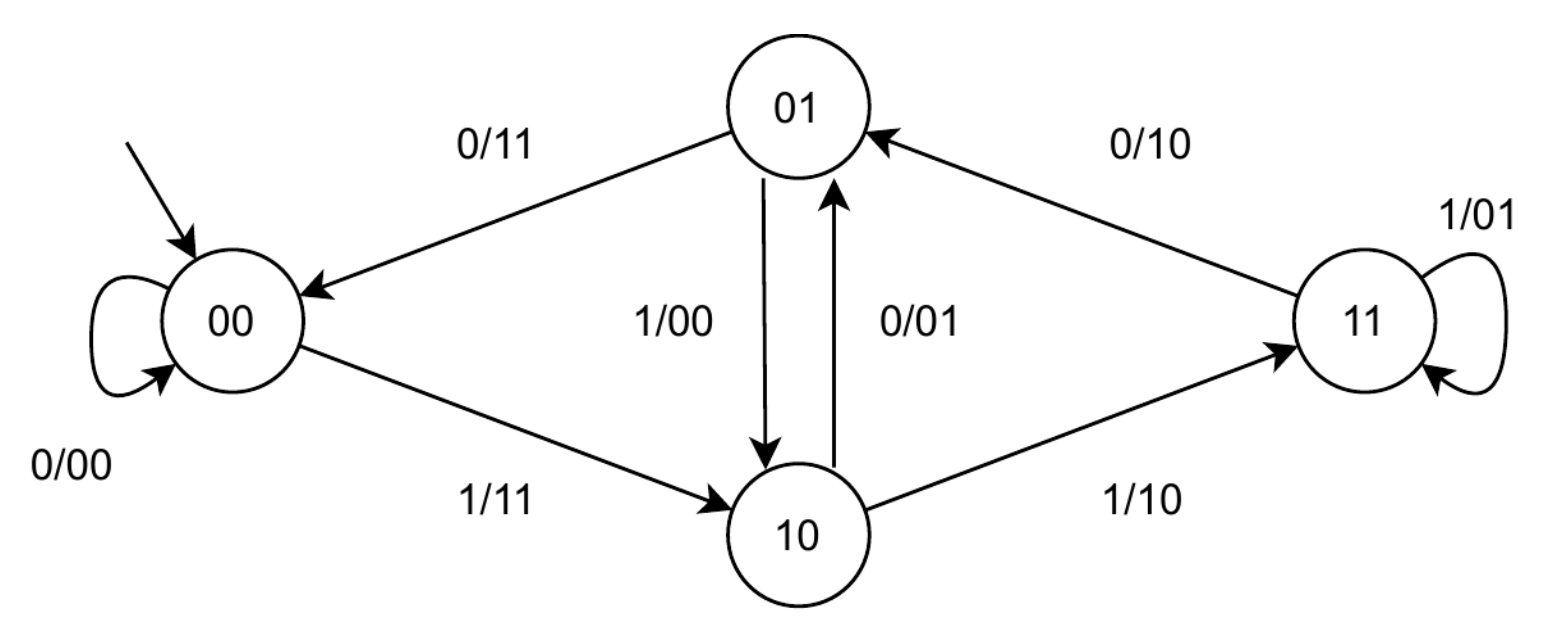
\includegraphics[scale=0.3]{./photo2.png}}
\end{center}

\subsection{Esempio di funzionamento} %1.4
\label{sec:esempio}
%Si riporta in seguito un esempio di elaborazione compiuta su un'immagine di test:

\begin{center}
    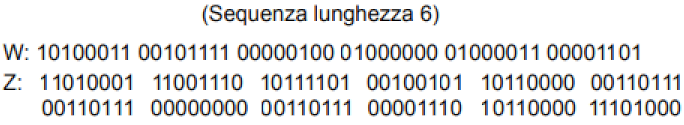
\includegraphics[scale=0.65]{./photo3.png}}
\end{center}
\begin{center}
    W \texttt{=} Input \texttt{|} Z \texttt{=} Output
\end{center}
\vspace{0,2cm}
\begin{table}[h]
    \centering
    \label{tab:esMEM}
    \begin{tabular}{c|c}
        addr. & data \\
        \hline \hline
        0     & 6    \\
        1     & 163  \\
        2     & 47   \\
        3     & 4    \\
        4     & 64   \\
        5     & 67   \\
        6     & 13   \\
        \texttt{[...]} &      \\ 
        1000  & 209  \\
        1001  & 206  \\
        1002  & 189  \\
        1003  & 37   \\
        1004  & 176  \\
        1005  & 55   \\
        1006  & 55   \\
        1007  & 0    \\
        1008  & 55   \\
        1009  & 14   \\
        1010  & 176  \\
        1011  & 232  \\
    \end{tabular}\hspace{15pt}
\end{table}

\pagebreak
\section{Architettura del componente} %2
Si è scelto di descrivere un modulo hardware tramite architettura \emph{behavioral} (comportamentale) in linguaggio VHDL.

\vspace{0,2cm}

\subsection{Macchina a stati finiti} %2.1
L’FSM schematizzata è composta da 13 stati descritti di seguito.
\subsubsection{Diagramma della macchina a stati finiti}
%immagine FSM
\begin{figure}[ht]
    \centering
    \begin{tikzpicture}[->,>=stealth',shorten >=1pt,auto,node distance=3cm, semithick, initial text=$ $, initial where= above]
        \node[state, initial]            (0) {\texttt{START}};
        \node[state, right of=0]         (1) {\texttt{WAIT}};
        \node[state, right of=1]         (2) {\texttt{READ\_0}};
        \node[state, right of=2]         (3) {\texttt{WAIT}};
        \node[state, below=4.5cm of 3]   (4) {\texttt{PREPARE}};
        \node[state, left of=4]          (5) {\texttt{WAIT}};
        \node[state, left of=5]          (6) {\texttt{READ\_BIT}};
        \node[state, below of=6]         (7) {\texttt{WAIT}};
        \node[state, left of=6]          (8) {\texttt{WRITE\_1}};
        \node[state, above of=8]         (9) {\texttt{WAIT}};
        \node[state, right of=9]         (10) {\texttt{WRITE\_2}};
        \node[state, right of=10]        (11) {\texttt{WAIT}};
        \node[state, below of=8]         (12) {\texttt{DONE}};

        \draw
        (0)  edge[loop left]      node {\texttt{i\_start=0}}             (0)
        (0)  edge                 node {\texttt{i\_start=1}}             (1)
        (1)  edge                 node {\texttt{}}                       (2)
        (2)  edge                 node {\texttt{}}                       (3)
        (3)  edge                 node {\texttt{}}                       (4)
        (4)  edge                 node {\texttt{}}                       (5)
        (5)  edge                 node {\texttt{}}                       (6)
        (6)  edge                 node {\texttt{\emph{cond3}}}           (7)
        (7)  edge                 node {\texttt{}}                       (6)
        (6)  edge                 node {\texttt{\emph{cond2}}}           (8)
        (8)  edge                 node {\texttt{}}                       (9)
        (9)  edge                 node {\texttt{}}                       (10)
        (10) edge                 node {\texttt{}}                       (11)
        (11) edge                 node {\texttt{}}                       (4)
        (6)  edge                 node {\texttt{\emph{cond1}}}           (12)
        (12) edge[loop left]      node {\texttt{i\_start=1}}             (12)
        (12) edge[bend left]      node {\texttt{i\_start=0}}             (0)
    \end{tikzpicture}
    \label{fig:fsm}
\end{figure}
\vspace{0,2cm}

In figura sono state utilizzate le seguenti abbreviazioni:
\vspace{-.1cm}
    \def\arraystretch{1.2} %un po' di padding
    \begin{tabular}{||c|c||}
        \hline
        \texttt{\emph{cond1}} & \texttt{to\_be\_processed = words\_processed}                  \\\hline
        \texttt{\emph{cond2}} & \texttt{!cond1 \& count = 8}                                   \\\hline
        \texttt{\emph{cond3}} & \texttt{!cond1 \& count != 8}                                  \\\hline
    \end{tabular}
\vspace{0,2cm}

Per ogni stato dell'FSM è presente un arco uscente implicito diretto verso lo stato di reset, che permette di interrompere in qualsiasi momento l'operazione corrente, tramite un segnale \texttt{i\_rst=1}.
\vspace{0,2cm}


\clearpage

\end{document}